\documentclass[11pt]{article}

% Fakesubsection Package imports and settings
\usepackage{amsmath}
\usepackage{amssymb}
\usepackage{array}
\usepackage{booktabs}
\usepackage[skip=12pt,labelfont=it,font=small]{caption}
\usepackage{float}
\usepackage{fullpage}
\usepackage{graphicx}
\usepackage[version=4]{mhchem}
\usepackage{multirow}
\usepackage{parskip}
\usepackage{setspace}
\usepackage{siunitx}
\usepackage{titlesec}
\usepackage{upgreek}
\usepackage{url}
\usepackage{xcolor}
\usepackage[hidelinks]{hyperref}
\floatplacement{figure}{!ht}
\floatplacement{table}{H}
\DeclareSIUnit{\molar}{\textsc{M}}
\DeclareSIUnit{\ppm}{ppm}
\doublespacing
% Fakesubsection Newcommands
\newcommand*{\carbon}{\ce{^{13}C}}
\newcommand*{\proton}{\ce{^{1}H}}
\newcommand*{\nitrogen}{\ce{^{15}N}}
\newcommand*{\red}[1]{\textcolor{red}{#1}}
\newcommand*{\onejxh}{{}^{1}\!J_{\ce{XH}}}
\newcommand*{\onejch}{{}^{1}\!J_{\ce{CH}}}
\newcommand*{\onejnh}{{}^{1}\!J_{\ce{NH}}}
\newcommand*{\jhh}{J_{\ce{HH}}}
\newcommand*{\figref}[1]{Figure \ref{fig:#1}}
\newcommand*{\tblref}[1]{Table \ref{tbl:#1}}
\newcommand*{\SInf}{\textit{Supporting Information}}
\newcommand*{\sitodo}{\red{(SI)}}
\newcommand*{\andro}{Spectra were obtained on a \SI{700}{\MHz} Bruker AV III equipped with a TCI H/C/N cryoprobe; the sample used was \SI{40}{\milli\molar} andrographolide in DMSO-$d_6$.}
\newcommand*{\grami}{Spectra were obtained on a \SI{700}{\MHz} Bruker AV III equipped with a TCI H/C/N cryoprobe; the sample used was \SI{40}{\milli\molar} gramicidin in DMSO-$d_6$.}
\newcommand*{\zolmi}{Spectra were obtained on a \SI{700}{\MHz} Bruker AV III equipped with a TCI H/C/N cryoprobe; the sample used was \SI{50}{\milli\molar} zolmitriptan in DMSO-$d_6$.}

% Fakesubsection Biblatex and reference sets
\usepackage[style=chem-acs,biblabel=dot,subentry]{biblatex}
\addbibresource{hsqc.bib}
% use "ref.\ (\citenum{REF_NAME})" to get "ref. (8)"
\DeclareCiteCommand{\citenum}{}{\printfield{labelnumber}}{}{}
\defbibentryset{ultrafast}{Frydman2002PNASUSA, Frydman2003JACS}
\defbibentryset{timeshared}{Nolis2007ACIE, Parella2010CMR}
\defbibentryset{multireceive}{Kupce2006JACS, Kovacs2016MRC}
\defbibentryset{noah}{Kupce2017ACIE, Kupce2018CC, Claridge2019MRC, Kupce2019JMR}
\defbibentryset{sehsqc}{Palmer1991JMR, Kay1992JACS, Cavanagh1993ARNMRS}
\defbibentryset{sehsqc_sens}{Schleucher1994JBNMR, Kontaxis1994JMR}
\defbibentryset{asaphsqc}{Schulze-Sunninghausen2014JACS, Schulze-Sunninghausen2017JMR}
\defbibentryset{ctphsqc}{Nolis2019CPC, Nolis2019JMR}

\begin{document}
% Fakesection Title, authors, affiliations
\begin{center}
    \Large \textbf{Diversifying NOAH Supersequences with New HSQC-Based Modules}

    \vspace{0.2cm}

    \large Jonathan R. J. Yong,\textsuperscript{1} {\=E}riks Kup{\v{c}}e,\textsuperscript{2} Tim D. W. Claridge\textsuperscript{1,}*

    \vspace{0.2cm}

    \normalsize

    \textsuperscript{1} \textit{Chemistry Research Laboratory, Department of Chemistry, University of Oxford, Mansfield Road, Oxford, OX1 3TA, U.K.}

    \textsuperscript{2} \textit{Bruker UK Ltd., Banner Lane, Coventry, CV4 9GH, U.K.}

    * \texttt{tim.claridge@chem.ox.ac.uk}
\end{center}

\vspace{0.5cm}

% Fakesection Abstract
\begin{abstract}
    The sensitivity-enhanced HSQC, as well as HSQC-TOCSY, experiments can be incorporated into NOAH (NMR by Ordered Acquisition using \proton{} detection) supersequences.
    Importantly, these heteronuclear modules preserve the magnetisation required for subsequent acquisition of other homonuclear modules in the supersequence.
    With these new modules, we reach a total of over 600 practically applicable NOAH supersequences which yield high-quality 2D spectra with greatly reduced experiment durations.
\end{abstract}

\section*{Introduction}

In recent years, there has been significant interest in techniques which accelerate the acquisition of NMR data, especially for multidimensional spectra.\autocite{ultrafast, timeshared, multireceive}
One of the most versatile approaches is to utilise different ``pools'' of magnetisation for the sequential collection of different spectra without an intervening recovery delay, as illustrated by the NOAH (NMR by Ordered Acquisition using \proton{} detection) technique.\autocite{noah}
Virtually all of the most common 2D experiments, such as HMBC, HSQC, COSY, NOESY, and TOCSY, can be concatenated in a modular fashion to form NOAH supersequences, providing time savings of up to $\sim 4\times$ as compared to individual acquisition of each spectrum.

One-bond heteronuclear correlation experiments, namely HMQC and HSQC, play a central role in the structural elucidation of small organic molecules and biomolecules.
\red{(cite)}
These experiments are also a core component of many NOAH experiments, since the magnetisation they use (protons directly coupled to dilute nuclei, i.e. \carbon{} and \nitrogen{}) can be efficiently differentiated from the ``bulk'' magnetisation of uncoupled protons.\autocite{Garbow1982CPL, Kupce2019JMR}
At the same time, due to the low natural abundance of these heteronuclei, these spectra are typically less sensitive than the homonuclear spectra that follow.
Consequently, for dilute samples, the minimum experimental time is generally dictated by these heteronuclear experiments.
Any improvements in experiment sensitivity can be translated into greater time savings.

In the 1990s, Cavanagh, Rance, and Kay introduced the sensitivity-enhanced HSQC (seHSQC) experiment, which improves on the sensitivity of an ordinary echo-antiecho HSQC by up to a factor of 2.\autocite{sehsqc}
This is accomplished by converting magnetisation that is both cosine- and sine-modulated in $t_1$ to observable magnetisation prior to detection, in the so-called preservation of equal pathways (PEP) scheme.
Here, we show how the original seHSQC sequence can be modified such that it can be used as a NOAH module.
We also introduce a HSQC-TOCSY module, derived from the ASAP-HSQC-TOCSY,\autocite{Becker2019JMR} that is also compatible with the NOAH strategy.
Both of these modules can be inserted either independently or together into NOAH supersequences, allowing large amounts of chemical information to be acquired in short times.

\section*{\texorpdfstring{\carbon{}}{13C} seHSQC}

\begin{figure}
    \centering
    % Inkscape
    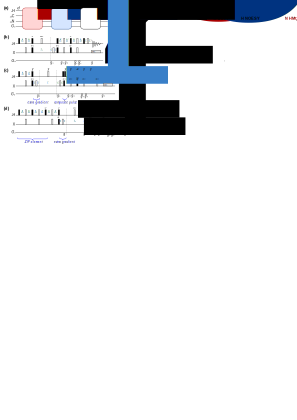
\includegraphics[width=0.7\textwidth]{./figures/pprogs.png}
    \caption{
        \textbf{(a)} Overview of a typical NOAH supersequence (MSCN, using the single-letter abbreviations previously defined\autocite{Kupce2017ACIE}).
        The \nitrogen{}--\proton{} HMQC and \carbon{}--\proton{} HSQC modules are highlighted: these may be replaced with the new seHSQC module proposed in this work.
        \textbf{(b)} Original NOAH HMQC module,\autocite{Kupce2017ACIE, Kupce2007MRC} abbreviated as ``M''.
        \textbf{(c)} Original NOAH HSQC module without sensitivity enhancement,\autocite{Kupce2017ACIE, Schulze-Sunninghausen2017JMR} abbreviated as ``S''.
        \textbf{(d)} Cavanagh--Rance--Kay (CRK) seHSQC.\autocite{sehsqc}
        \textbf{(e)} NOAH seHSQC module, abbreviated as ``Sp'' (this work).
        Filled and unfilled bars represent \ang{90} and \ang{180} pulses respectively; all \ang{180} pulses on \carbon{} are adiabatic (swept-frequency) pulses.
        All pulses are applied along $+x$ unless otherwise noted.
        The delays are chosen as follows: $\Delta = 1/(4\cdot\onejxh)$, $\Delta' = 1/(8\cdot\onejch)$ or $1/(4\cdot\onejnh)$, and $\varepsilon$ is the minimum time needed for a gradient and subsequent recovery.
        All gradients are \SI{1}{\ms} long, except for $g_1$ and $g_2$ in \nitrogen{} experiments which are \SI{2.5}{\ms} long.
        Gradient amplitudes, as percentages of maximum gradient strength, are as follows: $g_1 = 80\%$; $g_2 = \pm 40.2\%$ (\carbon{}) or $\pm 16.2\%$ (\nitrogen{}); ${g_2}' = g_2/2$; $g_3 = 11\%$; $g_4 = -5\%$.
        The signs of $g_2$ and ${g_2}'$ are alternated in each $t_1$ increment to provide echo--antiecho selection.
    }
    \label{fig:pprogs}
\end{figure}

NOAH supersequences, such as the MSCN experiment in \figref{pprogs}b, rely on the fact that the output of any one module contains all the necessary magnetisation components required for downstream modules.
The standard NOAH HSQC module (\figref{pprogs}c), derived from the symmetrised ASAP-HSQC,\autocite{asaphsqc} obeys this principle: it returns the ``bulk'' magnetisation belonging to uncoupled protons back to its equilibrium position ($+z$).
Introducing the sensitivity enhancement scheme, however, requires some extra care.
Using the original Cavanagh--Rance--Kay (CRK) seHSQC (\figref{pprogs}d) as part of a seHSQC/COSY NOAH supersequence, with the delay $\Delta'$ set to $1/(8 \cdot \onejch)$, affords sensitivity gains which are most significant for \ce{CH} peaks.\autocite{sehsqc_sens}
However, the CRK seHSQC also causes bulk magnetisation to be dephased by coherence transfer pathway (CTP) gradients.
Consequently, the downstream COSY can only utilise any bulk magnetisation that relaxes during the HSQC FID acquisition, leading to drastic intensity losses (\figref{spor_spv2}a).

\begin{figure}
    \centering
    % figures/spor_spv2_comp.py
    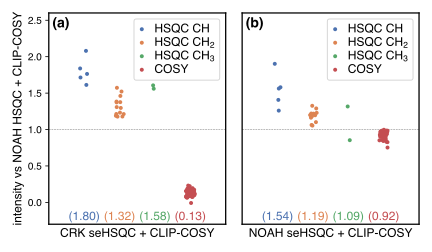
\includegraphics[width=0.6\textwidth]{figures/spor_spv2_comp.png}
    \caption{
        Sensitivity comparisons for seHSQC/CLIP-COSY\autocite{Koos2016ACIE} supersequences, using the CRK (\figref{pprogs}d) and NOAH (\figref{pprogs}e) seHSQC implementations.
        All intensities are normalised against a standard HSQC/CLIP-COSY supersequence (without sensitivity enhancement, i.e.\ \figref{pprogs}c).
        HSQC intensities are further split by multiplicity.
        Numbers in parentheses indicate averages over all peaks of a given type.
        \textbf{(a)} Using the original CRK seHSQC.
        The CRK seHSQC does not preserve the bulk magnetisation, leading to severely reduced COSY intensities.
        \textbf{(b)} Using the NOAH seHSQC.
        \andro{}
    }
    \label{fig:spor_spv2}
\end{figure}

Our solution is based on the simple observation that the bulk magnetisation in the seHSQC will be returned to $+z$ if the phase of the initial \proton{} \ang{90} pulse is changed to $+y$.
To generate the HSQC signal, however, the same pulse needs to be applied along $+x$.
Overall, what we need is therefore a pulse sequence element which simultaneously acts as a $90^\circ_x$ pulse on protons coupled to \carbon{}, and as a $90^\circ_y$ pulse on uncoupled protons.
We accomplish this by prepending two spin echoes, each of duration $2\Delta = 1/(2 \cdot \onejch)$, to the pulse sequence.
We refer to this element as an \textit{isotope-specific rotation} (ISR).
It is similar to the $zz$-filter used previously in the NOAH HMBC module,\autocite{Kupce2018CC, Kupce2019JMR} but has different pulse phases and thus leads to a different overall outcome.
The BIG-BIRD element developed by Briand and S{\o}rensen is also capable of effecting this;\autocite{Briand1997JMR} however, we find that the ISR provides better performance (\figref{bigbird}).

Apart from the ISR, the NOAH seHSQC module also contains an additional CTP gradient prior to the $t_1$ period (highlighted in \figref{pprogs}e).
This gradient is not necessary for the seHSQC module itself.
Instead, its purpose is to suppress artefacts in downstream modules, which arise from bulk magnetisation that evolves during either half of the HSQC $t_1$ period.
This then evolves again in the $t_1$ period of another homonuclear module (e.g.\ COSY).
Therefore, each COSY peak with $\Omega_1 = \Omega_{\ce{H}}$ is accompanied by a pair of ``wing'' artefacts at $\Omega_1 = \Omega_{\ce{H}} \pm (\Omega_{\ce{H}}\cdot\mathrm{SW}_{\ce{C}})/(2\cdot \mathrm{SW}_{\ce{H}})$, which can reach $\sim 5\%$ of the intensity of their parent peaks.
Importantly, the artefacts arising from diagonal peaks can have intensities that are comparable to genuine crosspeaks (\figref{wing_artefacts}), which highlights the importance of suppressing these artefacts.

With these modifications, the NOAH seHSQC module provides clear sensitivity gains over the NOAH HSQC module, while preserving essentially the same amount of magnetisation for downstream modules (\figref{spor_spv2}b).
The modifications present in the NOAH seHSQC, particularly the ISR, mean that the sensitivity improvements are slightly lower as compared to the original CRK implementation.
On average, \ce{CH} and \ce{CH2} peaks have 54\% and 19\% increased sensitivity respectively.
However, a dramatic improvement is seen in the COSY module which follows.
In contrast to the CRK seHSQC, which completely destroys the requisite bulk magnetisation, the NOAH seHSQC preserves the majority of it, performing 92\% as well as the original HSQC module.

Multiplicity editing can be easily incorporated into the NOAH seHSQC sequence (\figref{edited_sehsqc_pprog}), leading to similar sensitivity gains relative to the HSQC module.
It is noteworthy that the original NOAH HSQC (without sensitivity enhancement) places the bulk magnetisation in the $xy$-plane during the $t_1$ and editing periods, whereas the newly proposed NOAH seHSQC places the bulk along $\pm z$.
In the former, the bulk magnetisation is therefore subject to homonuclear coupling ($\jhh$) evolution, leading to a decrease in downstream sensitivity when multiplicity editing is introduced.
However, there is no such penalty in the NOAH seHSQC.
In fact, the edited NOAH seHSQC slightly \textit{outperforms} the edited HSQC in terms of preserving bulk magnetisation (\figref{edited_sn_comp}).

\red{Add a short section mentioning ASAP-seHSQC gains over standard ASAP-HSQC.}


\section*{\texorpdfstring{\nitrogen{}}{15N} seHSQC}

The proposed seHSQC module can be further extended to \nitrogen{} experiments.
Currently, in NOAH supersequences, \nitrogen{}--\proton{} correlations are primarily obtained using the HMQC module.\autocite{Kupce2007MRC, Kupce2017ACIE}
Compared to this, the new seHSQC module can provide up to $5\times$ greater sensitivity (\figref{n15}).
This arises partly because of the use of the PEP sensitivity enhancement scheme, in which the delays $\Delta'$ can be set to $1/(4 \cdot \onejnh)$ (i.e.\ optimised for \ce{NH} peaks).
However, there is also a significant improvement due to the fact that peaks in the seHSQC are not broadened in the indirect dimension by $\jhh$, unlike in the HMQC.
Although the seHSQC retains a slightly smaller amount of bulk magnetisation ($\sim 70\%$, versus $\sim 80\%$ for the HMQC), this is generally not a problem, since it is the \nitrogen{} module which typically has the lowest intrinsic sensitivity in a supersequence.

\begin{figure}
    \centering
    % figures/15n_spv2vsm.py
    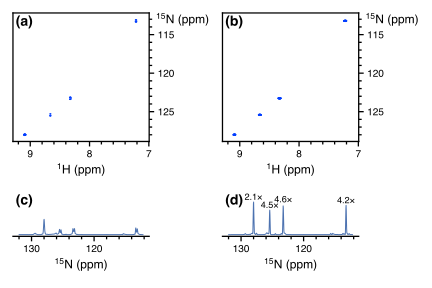
\includegraphics[width=0.6\textwidth]{./figures/15n_spv2vsm.png}
    \caption{
        Comparison of the new \nitrogen{}--\proton{} seHSQC with the standard NOAH HMQC module.
        \textbf{(a)} HMQC spectrum.
        \textbf{(b)} seHSQC spectrum.
        \textbf{(c)} Projection of HMQC onto the $f_1$ axis.
        Splitting due to $\jhh$ is clearly visible for three of the four peaks.
        \textbf{(d)} Projection of seHSQC onto the $f_1$ axis.
        Signal-to-noise improvements relative to the HMQC spectrum are indicated over each peak.
        The largest gains are observed for peaks where the multiplet structure is collapsed; however, even in the absence of that, a $\sim 2\times$ gain is still obtained.
        \grami{}
    }
    \label{fig:n15}
\end{figure}

While a \nitrogen{} HSQC module (without sensitivity enhancement) would still benefit from multiplet collapse, it comes with other severe drawbacks.
As previously discussed, the HSQC module places bulk magnetisation in the $xy$-plane during the $t_1$ period.
Consequently, due to $\jhh$ evolution, the amount of bulk magnetisation that is retained decreases as $t_1$ is lengthened, leading to line broadening in the indirect dimensions of all downstream modules (\figref{n15_linebroadening}).
This is not a problem with the \carbon{} HSQC, since typical \carbon{} indirect dimension acquisition times are relatively short.
However, with the smaller spectral widths in \nitrogen{} experiments, downstream modules can suffer substantial losses in sensitivity and resolution.

The \nitrogen{} seHSQC module has one major change with respect to its \carbon{} counterpart, which is that the CTP gradients $g_1$ and $g_2$ (\figref{pprogs}e) are all lengthened to \SI{2.5}{\ms}.
This is to effectively dephase any bulk magnetisation that is transverse just prior to detection, which can give rise to significant levels of artefacts in the seHSQC module itself.
The \carbon{} seHSQC does not need this because of the larger amplitude of $g_2$; however, the corresponding \nitrogen{} gradient is weaker by a factor of $\gamma_{\ce{C}}/\gamma_{\ce{N}} \approx 2.5$, thus requiring a longer duration in order to produce the same attenuation.
In practice, we find that gradient durations of 2 to \SI{2.5}{\ms} provide good artefact suppression.
These lengthened gradients do not cause any appreciable difference in the intensity of actual signals \sitodo{}.

In scenarios where high resolution in the \nitrogen{} dimension is not required, it can prove useful to reduce the number of $t_1$ increments and in its place increase the number of transients acquired.\autocite{Perez-Trujillo2007MRC, Parella2010CMR}
In new versions of the NOAH pulse programmes (including those provided in the \SInf{}), this feature can be enabled by specifying a factor $k$ by which to perform this scaling.
Note that the scaling is only applied to the \nitrogen{} module; all other modules are left untouched.
In our hands, setting $k = 2$ or 4 for the \nitrogen{} HMQC can lead to significant sensitivity gains \red{(how much?)}, since $\jhh$ splitting in the indirect dimension can no longer be resolved \sitodo{}.
This point is not relevant to the seHSQC, and here $k$-scaling on its own has only a tiny effect on peak height: any sensitivity gained from the extra transients is offset by the broadening.
However, the later $t_1$ increments which were not acquired can be reconstructed using linear projection \red{(cite)}.
The resulting spectra display sensitivity gains of up to a factor of $k$, although the fidelity of the reconstruction suffers for $k > 4$ \sitodo.

\section*{Double HSQC and HSQC-TOCSY}

\red{Need figure}

Next, we note that the HSQC module (though not the new seHSQC module) allows an arbitrary amount of \carbon{}--\proton{} magnetisation to be excited, with the remainder returned to $+z$.  In order to excite a proportion $f$ of \carbon{}--\proton{} magnetisation ($0 < f \leq 1$), the initial INEPT delay must be shortened by a factor of $\sin^{-1}f$.
The remaining $(1 - f)$ of the magnetisation, plus any that recovers during the first HSQC FID, can then be used for a second HSQC module in the same supersequence.
The collection of multiple HSQC spectra in one multi-FID acquisition (MFA) experiment has previously been accomplished by keeping the two CTPs in the CRK seHSQC separate, with the cosine- and sine-modulated CTPs each contributing to one spectrum.\autocite{ctphsqc}
However, with a value of $f = 0.7$, the NOAH strategy already provides slightly higher sensitivity for both spectra.
Furthermore, the sensitivity of the second HSQC can be further boosted by using the new seHSQC module in place of it \sitodo{}.

By adding a period of isotropic mixing prior to detection, the NOAH HSQC module may be converted to a HSQC-TOCSY module.
This is similar to the previously reported ASAP-HSQC-TOCSY,\autocite{Becker2019JMR} the key difference being that in the present NOAH context, unused \carbon{}--\proton{} and bulk magnetisation is preserved for use in other modules, instead of later $t_1$ increments as in the ASAP experiment.
Compared to the existing MFA HSQC-TOCSY/HSQC experiment,\autocite{Nolis2019CPC} our approach displays greater flexibility in three regards.
Firstly, the vast majority of bulk magnetisation is preserved, allowing for homonuclear module(s) to be appended in a NOAH supersequence (in practice, losses of ca.\ 10\% are observed due to pulse imperfections).
On the other hand, the MFA sequence, much like the original CRK seHSQC which it is based on, dephases bulk magnetisation and causes a 80--90\% sensitivity loss in downstream spectra.
Secondly, the sensitivity of both spectra can be optimised through the value of $f$; this allows a larger amount of \carbon{}--\proton{} magnetisation to be used for the inherently less sensitive HSQC-TOCSY (in our experience, setting $f = 0.9$ provides a good balance).
In contrast, isotropic mixing in the MFA sequence is applied to the less sensitive sine-modulated component, leading to spectra with imbalanced sensitivity.
Lastly, since each NOAH module is independently executed, the NOAH approach allows multiplicity editing to be enabled for only the HSQC and not the HSQC-TOCSY, where accidental overlap may lead to crosspeaks being lost unexpectedly.

Despite these benefits, it should be noted that the NOAH HSQC-TOCSY module will still have lower overall sensitivity than a conventional seHSQC-TOCSY, which can make use of the PEP scheme.
It is not possible to simply insert a TOCSY mixing block into the seHSQC module presented here, as that will lead to the bulk magnetisation being dephased.
As usual, the benefits of fast acquisition schemes such as NOAH are most obviously realised in sufficiently concentrated samples, where NMR data acquisition times are chiefly limited by the requisite number of $t_1$ increments.
In such settings, the same amount of data can be collected in much shorter times, without worrying about the slight loss in sensitivity inherent to all fast acquisition schemes.
On the other hand, for dilute samples where this sensitivity loss is less easily tolerated, the \textit{sensitivity per unit time} of each supersequence must then be taken into consideration.
As long as the time savings outweigh any sensitivity losses, use of the NOAH supersequence will then prove to be a net benefit.
Systematic investigations in this area will be detailed elsewhere.

\red{
    Assorted thoughts:
    \begin{enumerate}
        \item Do we need a figure illustrating the reduced delay and the HSQC-TOCSY pulse sequence? Should it be merged with the existing Fig 1, or Fig 4?
        \item I hope I have not been too critical of Parella's work. Everything I wrote \textit{is} true, and I want to say something positive about our work, but when that's the only real basis for comparison I feel like I might be being a bit harsh!
    \end{enumerate}
}

\section*{Example spectra and conclusion}

\begin{figure}
    \centering
    % figures/spstspcc.py
    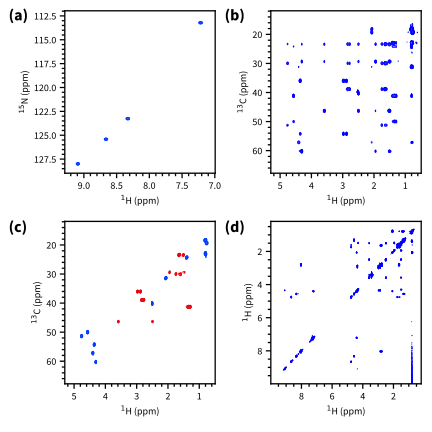
\includegraphics[width=0.6\textwidth]{figures/spstspcc.png}
    \caption{
        Example spectra obtained from the NOAH-4 SpStSpCc supersequence.
        256 $t_1$ increments were used, with 2 scans per increment.
        The total experiment time was 17 minutes and 35 seconds.
        \textbf{(a)} \nitrogen{} seHSQC.
        \textbf{(b)} \carbon{} HSQC-TOCSY ($f = 0.9$).
        \textbf{(c)} Multiplicity-edited \carbon{} seHSQC. Notice that having the edited seHSQC removes the need for the less desirable HSQC-TOCSY editing.
        \textbf{(d)} CLIP-COSY.
        \grami{}
    }
    \label{fig:example_spec}
\end{figure}

The NOAH-4 SpStSpCc (\nitrogen{} seHSQC, \carbon{} HSQC-TOCSY, \carbon{} seHSQC, and CLIP-COSY) supersequence is one of many ways in which the new modules discussed above can be included in practical experiments.
The spectra thus obtained are shown in \figref{example_spec}.
While individual collection of the four spectra above would require 57 minutes and 8 seconds, the NOAH-4 supersequence takes only 17 minutes and 35 seconds, which represents a $3.25\times$ speedup.
One can also prepend the NOAH HMBC module;\autocite{Kupce2019JMR} this uses the semi-adiabatic $zz$-filter to preserve magnetisation of protons directly coupled to \carbon{} and \nitrogen{} heteronuclei, which is precisely the magnetisation required by the HSQC-based modules presented here.
Examples of such spectra, with time savings of up to $3.8\times$, are shown in the \SInf{} \sitodo{}.

\red{Mention / emphasise BStSX type modules here -- applicable for typical organic molecules}

The new seHSQC and HSQC-TOCSY implementations add to the preexisting diversity in NOAH modules, bringing the total number of plausible NOAH supersequences to over 600.
The AU scripts needed for processing of these modules, as well as a number of the more commonly used pulse sequences, are provided in the \SInf{}; others are available upon request from the authors.
However, a more user-friendly and customisable method for the generation of NOAH pulse sequences is clearly needed to handle the sheer variety currently available.
Our work towards this will be reported in the near future.

\red{
    Final assorted thoughts:
    \begin{enumerate}
        \item We should probably provide ``new'' versions of pulse programmes here. The only thing that is backwards-\textit{incompatible} is the NUS implementation. Can we introduce that in the SI? [Perhaps just to avoid confusion, we should rename the new NUS script \texttt{noah\_nus2.py}?]
    \end{enumerate}
}


\section*{Acknowledgements}

J.R.J.Y.\ thanks the Clarendon Fund (University of Oxford) and the EPSRC Centre for Doctoral Training in Synthesis for Biology and Medicine (EP/L015838/1) for a studentship, generously supported by AstraZeneca, Diamond Light Source, Defence Science and Technology Laboratory, Evotec, GlaxoSmithKline, Janssen, Novartis, Pfizer, Syngenta, Takeda, UCB, and Vertex.
\red{Any other acknowledgements?}

% Fakesection Bibliography
\printbibliography

% Fakesection SI
% Fakesection Preamble-ish commands
\newcommand{\sectionbreak}{\clearpage}
\renewcommand\thefigure{S\arabic{figure}}
\renewcommand\thetable{S\arabic{table}}
\setcounter{page}{1}
\setcounter{figure}{0}
\setcounter{table}{0}
\onehalfspacing

% Fakesection Title page
\hspace{0pt}
\vfill
\begin{center}
    \huge
    Supporting Information

    \textit{for}

    Diversifying NOAH Supersequences with New HSQC-based Modules

    \vspace{1cm}

    \Large Jonathan R. J. Yong,\textsuperscript{1} {\=E}riks Kup{\v{c}}e,\textsuperscript{2} Tim D. W. Claridge\textsuperscript{1,}*

    \vspace{1cm}

    \large \textsuperscript{1} \textit{Chemistry Research Laboratory, Department of Chemistry, University of Oxford, Mansfield Road, Oxford, OX1 3TA, U.K.}

    \textsuperscript{2} \textit{Bruker UK Ltd., Banner Lane, Coventry, CV4 9GH, U.K.}

    * \texttt{tim.claridge@chem.ox.ac.uk}
\end{center}
\thispagestyle{empty}
\vfill
\hspace{0pt}
\newpage

% Fakesection Table of contents
\tableofcontents

\newpage

\section{Product operator analysis}

... 

\section{Multiplicity editing in seHSQC}

\begin{figure}
    \centering
    % done in Inkscape
    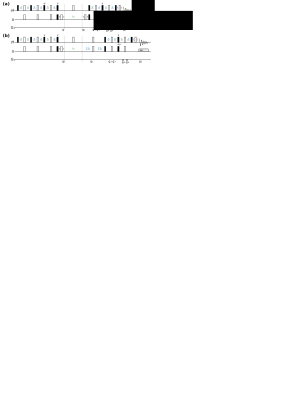
\includegraphics[width=0.8\textwidth]{./figures/mult_edit.png}
    \caption{
        Implementation of multiplicity editing in the new NOAH seHSQC module.
        \textbf{(a)} Unedited NOAH seHSQC, as presented in the main text.
        \textbf{(b)} Edited NOAH seHSQC (note the different phase in the third \proton{} \ang{90} pulse; this is needed to compensate for the extra \ang{180} in the editing period).
        Symbols have the same meaning as in \figref{pprogs} of the main text.
    }
    \label{fig:edited_sehsqc_pprog}
\end{figure}

\begin{figure}
    \centering
    % figures/edited_sn_comp.py
    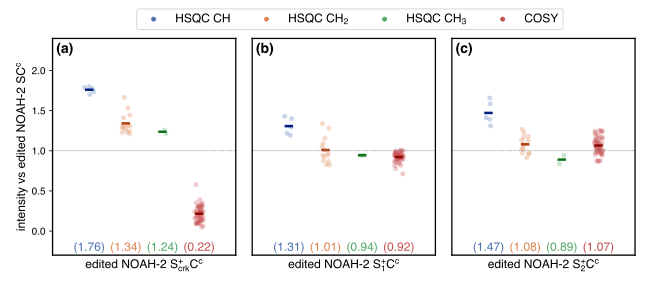
\includegraphics[width=0.8\textwidth]{./figures/edited_sn_comp.png}
    \caption{
        Sensitivity of edited seHSQC versus the NOAH HSQC/CLIP-COSY supersequence.
        \andro{}
        \textbf{(a)} CRK edited seHSQC + CLIP-COSY.
        Although larger gains are observed in the HSQC, the COSY intensities are severely decreased.
        \textbf{(b)} NOAH edited seHSQC + CLIP-COSY.
        On average, sensitivity gains are observed in both the HSQC and COSY modules (except for HSQC \ce{CH3} peaks).
    }
    \label{fig:edited_sn_comp}
\end{figure}

\section{Effect of setting \texorpdfstring{$\Delta' = 1/(4\cdot\onejch)$}{Delta' = 1/(4*1JCH)} in seHSQC}

The $\Delta'$ delay in the CRK and NOAH seHSQC sequences can be set to $1/(4\cdot\onejch)$ in order to optimise the sensitivity enhancement for \ce{CH} groups only.
The effects of doing so are shown here for the unedited and edited seHSQCs respectively.

\begin{figure}
    \centering
    % figures/combined_1_4j.py
    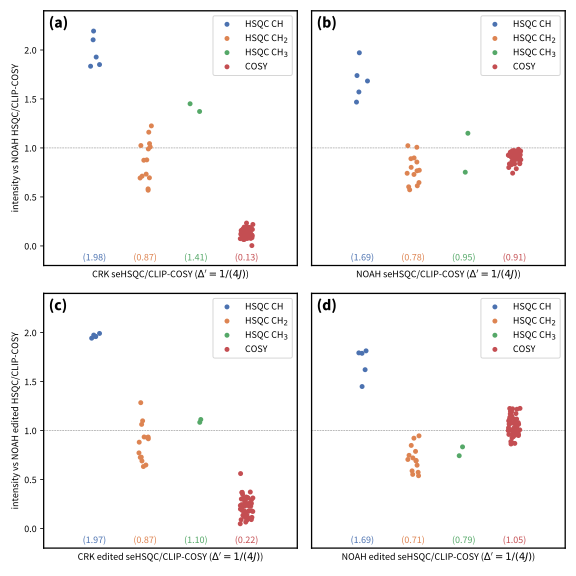
\includegraphics[width=0.8\textwidth]{./figures/combined_1_4j.png}
    \caption{
        Sensitivity of seHSQC sequences with $\Delta'$ set to $1/(4\cdot\onejch)$, versus the corresponding NOAH HSQC/CLIP-COSY supersequence (i.e.\ unedited for (a) and (b), edited for (c) and (d)).
        \andro{}
        \textbf{(a)} CRK seHSQC + CLIP-COSY, without multiplicity editing.
        \textbf{(b)} NOAH seHSQC + CLIP-COSY, without multiplicity editing.
        \textbf{(c)} CRK seHSQC + CLIP-COSY, with multiplicity editing.
        \textbf{(d)} NOAH seHSQC + CLIP-COSY, with multiplicity editing.
    }
    \label{fig:combined_1_4j}
\end{figure}

In particular, for the NOAH seHSQC, we note that the improvements in HSQC \ce{CH} sensitivity gained by moving from $\Delta' = 1/(8\cdot\onejch)$ to $\Delta' = 1/(4\cdot\onejch)$ are marginal (ca.\ 10\%).
At the same time, sensitivity \textit{losses} are observed for \ce{CH2} and \ce{CH3} peaks, likely due to pulse imperfections.

\section{Comparison of BIG-BIRD and ISR elements}

The BIG-BIRD element used here was ${45^\circ}_{45^\circ}(\proton{}) - 2\Delta - 180^\circ(\proton{},\carbon{}) - 2\Delta - {45^\circ}_{225^\circ}(\proton{})$ for the unedited NOAH seHSQC, where $\beta_\phi$ indicates a hard pulse with flip angle $\beta$ and phase $\phi$, and $\Delta = 1/(4\cdot\onejch)$.
For the edited NOAH seHSQC, the BIG-BIRD pulse phases are slightly modified to give ${45^\circ}_{315^\circ}(\proton{}) - 2\Delta - 180^\circ(\proton{},\carbon{}) - 2\Delta - {45^\circ}_{135^\circ}(\proton{})$.
These, and the ISR, have the same net effect on coupled and uncoupled proton magnetisation.
However, the ISR provides greater sensitivity in both the HSQC and downstream COSY.

\begin{figure}
    \centering
    % figures/bigbird.py
    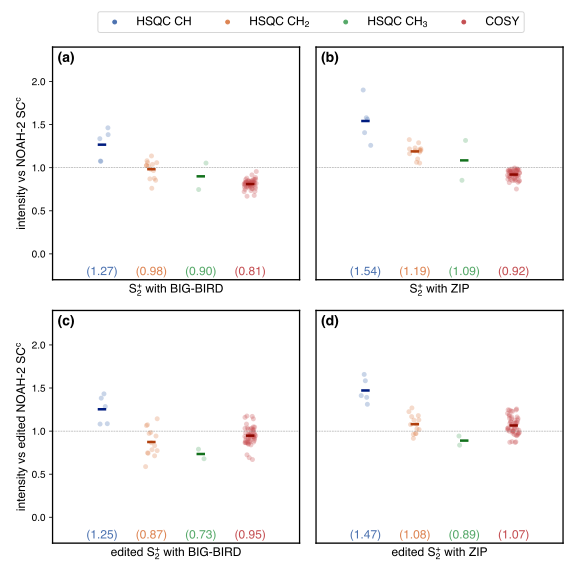
\includegraphics[width=0.8\textwidth]{./figures/bigbird.png}
    \caption{
        Sensitivity of NOAH seHSQC sequences with prepended BIG-BIRD and ISR elements, versus the corresponding NOAH HSQC/CLIP-COSY supersequence (i.e.\ unedited for (a) and (b), edited for (c) and (d)).
        \andro{}
        \textbf{(a)} NOAH seHSQC with BIG-BIRD + CLIP-COSY, without multiplicity editing.
        \textbf{(b)} NOAH seHSQC with ISR + CLIP-COSY, without multiplicity editing.
        \textbf{(c)} NOAH seHSQC with BIG-BIRD + CLIP-COSY, with multiplicity editing.
        \textbf{(d)} NOAH seHSQC with ISR + CLIP-COSY, with multiplicity editing.
    }
    \label{fig:bigbird}
\end{figure}


\section{Suppression of wing artefacts}

The origin of the ``wing'' artefacts in the final homonuclear modules can be most clearly seen from the following series of experiments involving the NOAH-3 \nitrogen{} seHSQC/\carbon{} seHSQC/CLIP-COSY (SpSpCc) supersequence.
Since the $f_1$ spectral windows of the two seHSQC modules are different, they lead to distinct sets of wing artefacts if the extra gradient before $t_1$ is not present.
\figref{wing_artefacts} focuses on the artefacts associated with intense methyl group peaks, but similar artefacts are observed for all other peaks, albeit with lower absolute intensities.

\begin{figure}
    \centering
    % figures/wing_artefacts.py
    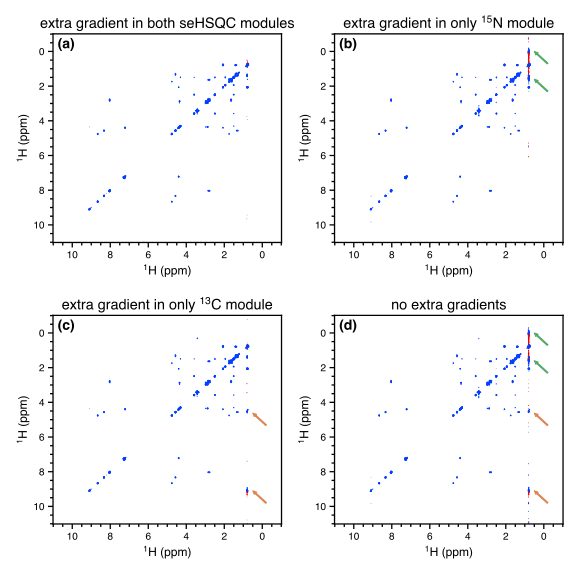
\includegraphics[width=0.8\textwidth]{./figures/wing_artefacts.png}
    \caption{
        CLIP-COSY spectra obtained from various forms of the NOAH-3 SpSpCc supersequence.
        Wing artefacts arising from the \nitrogen{} seHSQC are highlighted in orange; those arising from the \carbon{} seHSQC in green.
        Notice how (in this case) the former can easily be misinterpreted as a crosspeak, while the latter obscures genuine crosspeaks.
        \grami{}
        \textbf{(a)} With the extra gradient inserted for both modules, i.e.\ no artefacts.
        \textbf{(b)} With an extra gradient in only the \nitrogen{} module, i.e.\ only the \carbon{} artefacts.
        \textbf{(c)} With an extra gradient in only the \carbon{} module.
        \textbf{(d)} With no extra gradients.
    }
    \label{fig:wing_artefacts}
\end{figure}


\section{\texorpdfstring{\nitrogen{}}{15N} HSQC and line broadening}

For \nitrogen{}--\proton{} correlations, both the HMQC and the new seHSQC module are recommended as they keep the bulk magnetisation along $\pm z$ during the $t_1$ period.
The HSQC module places bulk magnetisation in the $xy$-plane, leading to $\jhh$ evolution; consequently, the amount of bulk magnetisation ``passed on'' to the downstream modules decreases as the \nitrogen{} $t_1$ is increased.
Since $t_1$ for each NOAH module is incremented in sync, this is manifested in downstream modules as a $t_1$-dependent decrease in amplitude, or $f_1$ line broadening after Fourier transformation, as shown in \figref{n15_linebroadening}.

\begin{figure}
    \centering
    % figures/n15_linebroadening.py
    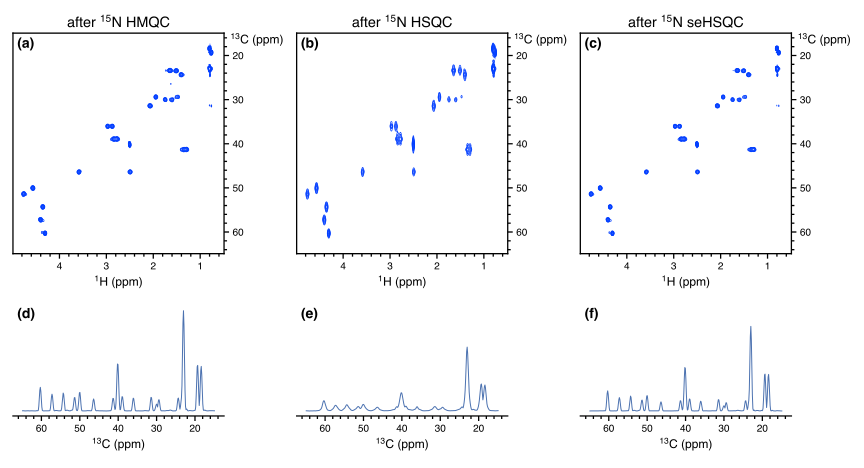
\includegraphics[width=\textwidth]{./figures/n15_linebroadening.png}
    \caption{
        \carbon{} seHSQC spectra obtained from NOAH-3 XSpCc (\nitrogen{} module + \carbon{} seHSQC + CLIP-COSY) supersequences.
        \grami{}
        The \nitrogen{} spectral window was \SI{30}{ppm} and 256 $t_1$ increments were collected, corresponding to an indirect-dimension \nitrogen{} acquisition time of \SI{60.1}{\ms}.
        \textbf{(a)} X = HMQC.
        \textbf{(b)} X = HSQC.
        \textbf{(c)} X = seHSQC.
        \textbf{(d)}--\textbf{(f)} Projections of spectra \textbf{(a)}--\textbf{(c)} onto the $f_1$ axis.
        Note the $f_1$ line broadening in (b) and (e).
    }
    \label{fig:n15_linebroadening}
\end{figure}

This line broadening also leads to a substantial sensitivity loss (almost 65\% in \figref{n15_linebroadening}).
The extent of the line broadening depends on the acquisition time, and is particularly pronounced for long acquisition times, i.e.\ small \nitrogen{} spectral windows.
In our experience, at \nitrogen{} acquisition times of ca.\ \SI{5}{\ms} the effect is almost indiscernible.
Such a short acquisition time would lead to poor resolution in the \nitrogen{} dimension itself, which may or may not be tolerable.
Of course, this issue can be entirely avoided by using either the HMQC or seHSQC.

\section{Effect of lengthened gradients in \texorpdfstring{\nitrogen{}}{15N} experiments}

cnst16 scan

\section{Effect of \texorpdfstring{$k$}{k}-scaling}

... both signal and artefact intensity, plus example spectra

\section{HSQC-TOCSY SNR comparisons}

... including Parella work

\section{Other example spectra}

...

\section{Pulse programmes}

...

\section{Processing scripts}

...


\end{document}
